\chapter{System Process}

As each new sample (theta, delta, epsilon, jitter, t) is produced by
the clock filter algorithm, all peer processes are scanned by the
mitigation algorithms consisting of the selection, cluster, combine,
and clock discipline algorithms in the system process.  The selection
algorithm scans all associations and casts off the falsetickers,
which have demonstrably incorrect time, leaving the truechimers as
result.  In a series of rounds, the cluster algorithm discards the
association statistically furthest from the centroid until a
specified minimum number of survivors remain.  The combine algorithm
produces the best and final statistics on a weighted average basis.
The final offset is passed to the clock discipline algorithm to steer
the system clock to the correct time.

The cluster algorithm selects one of the survivors as the system
peer.  The associated statistics (theta, delta, epsilon, jitter, t)
are used to construct the system variables inherited by dependent
servers and clients and made available to other applications running
on the same machine.

\section{System Process Variables}

Figure 23 summarizes the common names, formula names, and a short
description of each system variable.  Unless noted otherwise, all
variables have assumed prefix s.

\begin{table}[htb]
\center
\begin{tabular}{c | c | c}
Name & Formula & Description \\
\hline
\hline
t         & t          & update time            \\
p         & p          & system peer identifier \\
leap      & leap       & leap indicator         \\
stratum   & stratum    & stratum                \\
precision & rho        & precision              \\
offset    & THETA      & combined offset        \\
jitter    & PSI        & combined jitter        \\
rootdelay & DELTA      & root delay             \\
rootdisp  & EPSILON    & root dispersion        \\
v         & v          & survivor list          \\
refid     & refid      & reference ID           \\
reftime   & reftime    & reference time         \\
NMIN      & 3          & minimum survivors      \\
CMIN      & 1          & minimum candidates     \\
\hline
\end{tabular}
\label{system_process_variables}
\caption{System Process Variables}
\end{table}

Except for the t, p, offset, and jitter variables and the NMIN and
CMIN constants, the variables have the same format and interpretation
as the peer variables of the same name.  The NMIN and CMIN parameters
are used by the selection and cluster algorithms described in the
next section.

The t variable is the seconds counter at the time of the last update.
An example is shown by the clock\_update() routine in
Appendix A.5.5.4.  The p variable is the system peer identifier
determined by the cluster() routine in Section 11.2.2.  The precision
variable has the same format as the packet variable of the same name.
The precision is defined as the larger of the resolution and time to
read the clock, in log2 units.  For instance, the precision of a
mains-frequency clock incrementing at 60 Hz is 16 ms, even when the
system clock hardware representation is to the nanosecond.

The offset and jitter variables are determined by the combine
algorithm in Section 11.2.3.  These values represent the best and
final offset and jitter used to discipline the system clock.
Initially, all variables are cleared to zero, then the leap is set to
3 (unsynchronized) and stratum is set to MAXSTRAT (16).  Remember
that MAXSTRAT is mapped to zero in the transmitted packet.

\section{System Process Operations}

Figure 24 summarizes the system process operations performed by the
clock select routine.  The selection algorithm described in
Section 11.2.1 produces a majority clique of presumed correct
candidates (truechimers) based on agreement principles.  The cluster
algorithm described in Section 11.2.2 discards outliers to produce
the most accurate survivors.  The combine algorithm described in
Section 11.2.3 provides the best and final offset for the clock
discipline algorithm.  An example is described in Appendix A.5.5.6.
If the selection algorithm cannot produce a majority clique, or if it
cannot produce at least CMIN survivors, the system process exits
without disciplining the system clock.  If successful, the cluster
algorithm selects the statistically best candidate as the system peer
and its variables are inherited as the system variables.

\begin{figure}
\centering
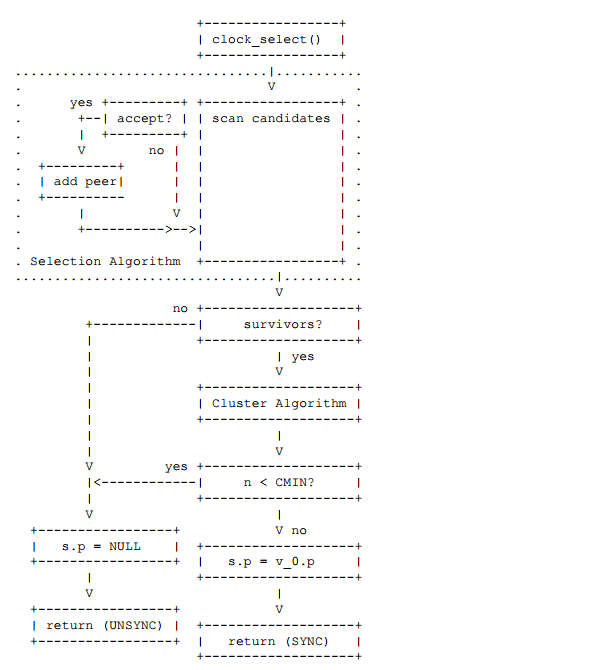
\includegraphics[width=\textwidth]{clock_select_routine.png}
\caption{Clock Select Routine}
\label{clock_select_routine}
\end{figure}

\section{Selection Algorithm}

Note that the selection and cluster algorithms are described
separately, but combined in the code skeleton.  The selection
algorithm operates to find an intersection interval containing a
majority clique of truechimers using Byzantine agreement principles
originally proposed by Marzullo \cite{ref6}, but modified to improve
accuracy.  An overview of the algorithm is given below and described
in the first half of the clock\_select() routine in Appendix A.5.5.1.

First, those servers that are unusable according to the rules of the
protocol are detected and discarded as shown by the accept() routine
in Appendix A.5.5.3.  Next, a set of tuples (p, type, edge) is
generated for the remaining candidates.  Here, p is the association
identifier and type identifies the upper (+1), middle (0), and lower
(-1) endpoints of a correctness interval centered on theta for that
candidate.  This results in three tuples, lowpoint (p, -1, theta -
lambda), midpoint (p, 0, theta), and highpoint (p, +1, theta +
lambda), where lambda is the root synchronization distance.  An
example of this calculation is shown by the rootdist() routine in
Appendix A.5.1.1.  The steps of the algorithm are:

\begin{enumerate}
  \item For each of m associations, place three tuples as defined above
    on the candidate list.

  \item Sort the tuples on the list by the edge component.  Order the
    lowpoint, midpoint, and highpoint of these intervals from lowest to
    highest.  Set the number of falsetickers f = 0.

  \item Set the number of midpoints d = 0.  Set c = 0.  Scan from lowest
    endpoint to highest.  Add one to c for every lowpoint, subtract one
    for every highpoint, add one to d for every midpoint.  If c >= m - f,
    stop; set l = current lowpoint.

  \item Set c = 0.  Scan from highest endpoint to lowest.  Add one to c
    for every highpoint, subtract one for every lowpoint, add one to d
    for every midpoint.  If c >= m - f, stop; set u = current highpoint.

  \item Is d = f and l < u?  If yes, then follow step 5A; else, follow
    step 5B.

    \begin{enumerate}[5A.]
      \item Success: the intersection interval is [l, u].

      \item Add one to f.  Is f < (m / 2)?  If yes, then go to step 3 again.
        If no, then go to step 6.
    \end{enumerate}

  \item Failure; a majority clique could not be found.  There are no
    suitable candidates to discipline the system clock.
    The algorithm is described in detail in Appendix A.5.5.1.  Note that
    it starts with the assumption that there are no falsetickers (f = 0)
    and attempts to find a non-empty intersection interval containing the
    midpoints of all correct servers, i.e., truechimers.  If a non-empty
    interval cannot be found, it increases the number of assumed
    falsetickers by one and tries again.  If a non-empty interval is
    found and the number of falsetickers is less than the number of
    truechimers, a majority clique has been found and the midpoint of
    each truechimer (theta) represents the candidates available to the
    cluster algorithm.

    If a majority clique is not found, or if the number of truechimers is
    less than CMIN, there are insufficient candidates to discipline the
    system clock.  CMIN defines the minimum number of servers consistent
    with the correctness requirements.  Suspicious operators would set
    CMIN to ensure multiple redundant servers are available for the
    algorithms to mitigate properly.  However, for historic reasons the
    default value for CMIN is one.
\end{enumerate}

\section{Cluster Algorithm}

The candidates of the majority clique are placed on the survivor list
v in the form of tuples (p, theta\_p, psi\_p, lambda\_p), where p is an
association identifier, theta\_p, psi\_p, and stratum\_p the current
offset, jitter and stratum of association p, respectively, and
lambda\_p is a merit factor equal to stratum\_p * MAXDIST + lambda,
where lambda is the root synchronization distance for association p.
The list is processed by the cluster algorithm below.  An example is
shown by the second half of the clock\_select() algorithm in
Appendix A.5.5.1.

\begin{enumerate}
  \item Let (p, theta\_p, psi\_p, lambda\_p) represent a survivor candidate.

  \item Sort the candidates by increasing lambda\_p.  Let n be the number
    of candidates and NMIN the minimum required number of survivors.

  \item For each candidate, compute the selection jitter psi\_s:

    $$
    \psi_s = \left( \frac{1}{n - 1} \cdot \sum^{n - 1}_{j = 1} (\theta_s - \theta_j)^2 \right)^{\frac{1}{2}}
    $$

  \item Select psi\_max as the candidate with maximum psi\_s.
  \item Select psi\_min as the candidate with minimum psi\_p.

  \item Is psi\_max < psi\_min or n <= NMIN?  If yes, follow step 6A;
    otherwise, follow step 6B.

    \begin{enumerate}[6A.]
      \item Done. The remaining candidates on the survivor list are ranked
      in the order of preference.  The first entry on the list represents
      the system peer; its variables are used later to update the system
      variables.

      \item Delete the outlier candidate with psi\_max; reduce n by one and go
      back to step 3.
    \end{enumerate}
\end{enumerate}

The algorithm operates in a series of rounds where each round
discards the statistical outlier with maximum selection jitter psi\_s.
However, if psi\_s is less than the minimum peer jitter psi\_p, no
improvement is possible by discarding outliers.  This and the minimum
number of survivors represent the terminating conditions of the
algorithm.  Upon termination, the final value of psi\_max is saved as
the system selection jitter PSI\_s for use later.

\section{Combine Algorithm}

The clock combine route processes the remaining survivors to produce
the best and final data for the clock discipline algorithm.  The
routine processes peer offset and jitter statistics to produce the
combined system offset THETA and system peer jitter PSI\_p, where each
server statistic is weighted by the reciprocal of the root
synchronization distance and the result normalized.  An example is
shown by the clock\_combine() routine in Appendix A.5.5.5

The combined THETA is passed to the clock update routine.  The first
candidate on the survivor list is nominated as the system peer with
identifier p.  The system peer jitter PSI\_p is a component of the
system jitter PSI.  It is used along with the selection jitter PSI\_s
to produce the system jitter:

$$
\Psi = \left( \Psi_s^2 + \Psi_p^2 \right)^{\frac{1}{2}}
$$

Each time an update is received from the system peer, the clock
update routine is called.  By rule, an update is discarded if its
time of arrival p.t is not strictly later than the last update used
s.t.  The labels IGNOR, PANIC, ADJ, and STEP refer to return codes
from the local clock routine described in the next section.

IGNORE means the update has been ignored as an outlier.  PANIC means
the offset is greater than the panic threshold PANICT (1000 s) and
SHOULD cause the program to exit with a diagnostic message to the
system log.  STEP means the offset is less than the panic threshold,
but greater than the step threshold STEPT (125 ms).  In this case,
the clock is stepped to the correct offset, but since this means all
peer data have been invalidated, all associations MUST be reset and
the client begins as at initial start.

ADJ means the offset is less than the step threshold and thus a valid
update.  In this case, the system variables are updated from the peer
variables as shown in Figure 25.

\begin{table}[htb]
\center
\begin{tabular}{c | c | c}
System Variable & <-- & System Peer Variable \\
\hline
\hline
s.leap      & <-- & p.leap                    \\
s.stratum   & <-- & p.stratum + 1             \\
s.offset    & <-- & THETA                     \\
s.jitter    & <-- & PSI                       \\
s.rootdelay & <-- & p.delta\_r + delta         \\
s.rootdisp  & <-- & p.epsilon\_r + p.epsilon + p.psi + PHI * (s.t - p.t) + |THETA|  \\
s.refid     & <-- & p.refid                   \\
s.reftime   & <-- & p.reftime                 \\
s.t         & <-- & p.t                       \\
\hline
\end{tabular}
\label{system_variables_update}
\caption{System Variables Update}
\end{table}

There is an important detail not shown.  The dispersion increment
(p.epsilon + p.psi + PHI * (s.t - p.t) + |THETA|) is bounded from
below by MINDISP.  In subnets with very fast processors and networks
and very small delay and dispersion this forces a monotone-definite
increase in s.rootdisp (EPSILON), which avoids loops between peers
operating at the same stratum.

The system variables are available to dependent application programs
as nominal performance statistics.  The system offset THETA is the
clock offset relative to the available synchronization sources.  The
system jitter PSI is an estimate of the error in determining this
value, elsewhere called the expected error.  The root delay DELTA is
the total round-trip delay relative to the primary server.  The root
dispersion EPSILON is the dispersion accumulated over the network
from the primary server.  Finally, the root synchronization distance
is defined as:

$$
\Lambda = E + \frac{\Delta}{2},
$$

which represents the maximum error due all causes and is designated
the root synchronization distance.

An example of the clock update routine is provided in
Appendix A.5.5.4.

\section{Clock Discipline Algorithm}

The NTPv4 clock discipline algorithm, shortened to discipline in the
following, functions as a combination of two quite philosophically
different feedback control systems.  In a phase-locked loop (PLL)
design, periodic phase updates at update intervals mu seconds are
used directly to minimize the time error and indirectly the frequency
error.  In a frequency-locked loop (FLL) design, periodic frequency
updates at intervals mu are used directly to minimize the frequency
error and indirectly the time error.  As shown in \cite{ref7}, a PLL
usually works better when network jitter dominates, while an FLL
works better when oscillator wander dominates.  This section contains
an outline of how the NTPv4 design works.  An in-depth discussion of
the design principles is provided in \cite{ref7}, which also includes a
performance analysis.

The discipline is implemented as the feedback control system shown in
Figure 26.  The variable theta\_r represents the combine algorithm
offset (reference phase) and theta\_c the VFO offset (control phase).
Each update produces a signal V\_d representing the instantaneous
phase difference theta\_r - theta\_c.  The clock filter for each server
functions as a tapped delay line, with the output taken at the tap
selected by the clock filter algorithm.  The selection, cluster, and
combine algorithms combine the data from multiple filters to produce
the signal V\_s.  The loop filter, with impulse response F(t),
produces the signal V\_c, which controls the VFO frequency omega\_c and
thus the integral of the phase theta\_c which closes the loop.  The
V\_c signal is generated by the clock-adjust process in Section 12.
The detailed equations that implement these functions are best
presented in the routines of Appendices A.5.5.6 and A.5.6.1.

\begin{figure}
\centering
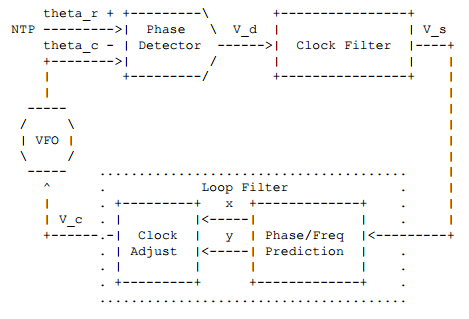
\includegraphics[width=\textwidth]{clock_discipline_feedback_loop.png}
\caption{Clock Discipline Feedback Loop}
\label{clock_discipline_feedback_loop}
\end{figure}

Ordinarily, the pseudo-linear feedback loop described above operates
to discipline the system clock.  However, there are cases where a
non-linear algorithm offers considerable improvement.  One case is
when the discipline starts without knowledge of the intrinsic clock
frequency.  The pseudo-linear loop takes several hours to develop an
accurate measurement and during most of that time the poll interval
cannot be increased.  The non-linear loop described below does this
in 15 minutes.  Another case is when occasional bursts of large
jitter are present due to congested network links.  The state machine
described below resists error bursts lasting less than 15 minutes.

Figure 27 contains a summary of the variables and parameters
including the variable (lowercase) or parameter (uppercase) name,
formula name, and short description.  Unless noted otherwise, all
variables have assumed prefix c.  The variables t, tc, state, hyster,
and count are integers; the remaining variables are floating doubles.
The function of each will be explained in the algorithm descriptions
below.

\begin{table}[htb]
\center
\begin{tabular}{c | c | c}
Name   | Formula    | Description              \\
\hline
\hline
t      & timer      & seconds counter          \\
offset & theta      & combined offset          \\
resid  & theta\_r   & residual offset          \\
freq   & phi        & clock frequency          \\
jitter & psi        & clock offset jitter      \\
wander & omega      & clock frequency wander   \\
tc     & tau        & time constant (log2)     \\
state  & state      & state                    \\
adj    & adj        & frequency adjustment     \\
hyster & hyster     & hysteresis counter       \\
STEPT  & 125        & step threshold (.125 s)  \\
WATCH  & 900        & stepout thresh(s)        \\
PANICT & 1000       & panic threshold (1000 s) \\
LIMIT  & 30         & hysteresis limit         \\
PGATE  & 4          & hysteresis gate          \\
TC     & 16         & time constant scale      \\
AVG    & 8          & averaging constant       \\
\hline
\end{tabular}
\label{clock_discipline_variables_and_parameters}
\caption{Clock Discipline Variables and Parameters}
\end{table}

The process terminates immediately if the offset is greater than the
panic threshold PANICT (1000 s).  The state transition function is
described by the rstclock() function in Appendix A.5.5.7.  Figure 28
shows the state transition function used by this routine.  It has
four columns showing, respectively, the state name, predicate and
action if the offset theta is less than the step threshold, the
predicate and actions otherwise, and finally some comments.

\begin{table}[htb]
\center
\begin{tabular}{c | c | c | c}
State & theta < STEP        & theta > STEP      & Comments \\
\hline
\hline
NSET & \makecell{->FREQ \\ adjust time} & \makecell{->FREQ \\ step time} & no frequency file \\
FSET & \makecell{->SYNC \\ adjust time} & \makecell{->SYNC \\ step time} & frequency file \\
SPIK & \makecell{->SYNC \\ adjust freq \\ adjust time} & \makecell{if < 900 s ->SPIK \\ else ->SYNC \\ step freq \\ step time} & outlier detected \\
FREQ & \makecell{if < 900 s ->FREQ \\ else ->SYNC \\ step freq \\ adjust time} & \makecell{if < 900 s ->FREQ \\ else ->SYNC \\ step freq \\ adjust time} & initial frequency \\
SYNC & \makecell{->SYNC \\ adjust freq \\ adjust time} & \makecell{if < 900 s ->SPIK \\ else ->SYNC \\ step freq \\ step time} & normal operation \\
\hline
\end{tabular}
\label{state_transition_function}
\caption{State Transition Function}
\end{table}

In the table entries, the next state is identified by the arrow ->
with the actions listed below.  Actions such as adjust time and
adjust frequency are implemented by the PLL/FLL feedback loop in the
local\_clock() routine.  A step clock action is implemented by setting
the clock directly, but this is done only after the stepout threshold
WATCH (900 s) when the offset is more than the step threshold STEPT
(.125 s).  This resists clock steps under conditions of extreme
network congestion.

The jitter (psi) and wander (omega) statistics are computed using an
exponential average with weight factor AVG.  The time constant
exponent (tau) is determined by comparing psi with the magnitude of
the current offset theta.  If the offset is greater than PGATE (4)
times the clock jitter, the hysteresis counter hyster is reduced by
two; otherwise, it is increased by one.  If hyster increases to the
upper limit LIMIT (30), tau is increased by one; if it decreases to
the lower limit -LIMIT (-30), tau is decreased by one.  Normally, tau
hovers near MAXPOLL, but quickly decreases if a temperature spike
causes a frequency surge.
